\documentclass{article}
\usepackage{ifluatex}
\ifluatex 
    \usepackage{fontspec}
    \setsansfont[
        Path = C:/Windows/Fonts/,
        Extension = .ttf ,
        BoldFont={cmunsx} ,
        ItalicFont={cmunsi} ,
        BoldItalicFont={cmunso} ,
        UprightFont={cmunss}
    ]{CMU Sans Serif}
    \setmainfont[
        Path = C:/Windows/Fonts/,
        Extension = .ttf ,
        BoldItalicFont={cmunbi} ,
        ItalicFont={cmunti} ,
        BoldFont={cmunbx} ,
        UprightFont={cmunrm}
    ]{CMU Serif}
    \setmonofont[
        Path = C:/Windows/Fonts/,
        Extension = .ttf ,
        % LightFont={cmunbtl} ,
        BoldItalicFont={cmuntx} ,
        % LightItalicFont={cmunbto} ,
        BoldFont={cmuntb} ,
        ItalicFont={cmunit} ,
        UprightFont={cmuntt}
    ]{CMU Typewriter Text}
    \defaultfontfeatures{Ligatures={TeX}}
\else
    \usepackage[T2A]{fontenc}
    \usepackage[utf8]{inputenc}
\fi
\usepackage[english,russian]{babel}
\usepackage{anyfontsize}
\usepackage{amssymb,latexsym,amsmath,amscd,mathtools,wasysym,stmaryrd}
\usepackage[shortlabels]{enumitem}
\usepackage[makeroom]{cancel}
\usepackage{graphicx}
\usepackage{geometry}
\usepackage{verbatim}
\usepackage{fvextra}

\usepackage{longtable}
\usepackage{multirow}
\usepackage{multicol}
\usepackage{tabu}
\usepackage{arydshln} % \hdashline and :
\usepackage{makecell} % \makecell for line breaks
\usepackage{tabularx}
\usepackage{xltabular}
\renewcommand\tabularxcolumn[1]{m{#1}} % for vertical centering text in X column


\usepackage{float}
\makeatletter
\g@addto@macro\@floatboxreset\centering
\makeatother
\setlength{\parindent}{0pt}
\usepackage{caption}
\usepackage{csquotes}
\usepackage[bb=dsserif]{mathalpha}
\usepackage[normalem]{ulem}

\usepackage[e]{esvect}
\let\vec\vv

\usepackage[x11names]{xcolor}
\colorlet{darkgreen}{black!25!blue!50!green}


%% Here f*cking with mathabx
\DeclareFontFamily{U}{matha}{\hyphenchar\font45}
\DeclareFontShape{U}{matha}{m}{n}{
    <5> <6> <7> <8> <9> <10> gen * matha
    <10.95> matha10 <12> <14.4> <17.28> <20.74> <24.88> matha12
}{}
\DeclareSymbolFont{matha}{U}{matha}{m}{n}
\DeclareFontFamily{U}{mathb}{\hyphenchar\font45}
\DeclareFontShape{U}{mathb}{m}{n}{
    <5> <6> <7> <8> <9> <10> gen * mathb
    <10.95> matha10 <12> <14.4> <17.28> <20.74> <24.88> mathb12
}{}
\DeclareSymbolFont{mathb}{U}{mathb}{m}{n}

\DeclareMathSymbol{\tmp}{\mathrel}{mathb}{"15}
\let\defeq\tmp
\DeclareMathSymbol{\tmp}{\mathrel}{mathb}{"16}
\let\eqdef\tmp

\usepackage{trimclip}
\DeclareMathOperator{\updownarrows}{\clipbox{0pt 0pt 4.175pt 0pt}{$\upuparrows$}\hspace{-.825px}\clipbox{0pt 0pt 4.175pt 0pt}{$\downdownarrows$}}
\DeclareMathOperator{\downuparrows}{\clipbox{0pt 0pt 4.175pt 0pt}{$\downdownarrows$}\hspace{-.825px}\clipbox{0pt 0pt 4.175pt 0pt}{$\upuparrows$}}

\makeatletter
\providecommand*\deletecounter[1]{%
    \expandafter\let\csname c@#1\endcsname\@undefined}
\makeatother


\usepackage{hyperref}
\hypersetup{
    %hidelinks,
    colorlinks=true,
    linkcolor=darkgreen,
    urlcolor=blue,
    breaklinks=true,
}

\usepackage{pgf}
\usepackage{pgfplots}
\pgfplotsset{compat=newest}
\usepackage{tikz,tikz-3dplot}
\usepackage{tkz-euclide}
\usetikzlibrary{calc,automata,patterns,angles,quotes,backgrounds,shapes.geometric,trees,positioning,decorations.pathreplacing}
\usetikzlibrary{lindenmayersystems}
\pgfkeys{/pgf/plot/gnuplot call={cd Output && gnuplot}}
\usepgfplotslibrary{fillbetween,polar}
\usetikzlibrary{quotes,babel}
\ifluatex
\usetikzlibrary{graphs,graphs.standard,graphdrawing}
\usegdlibrary{layered,trees,circular,force}
\else
% \errmessage{Run with LuaTeX, if you want to use gdlibraries}
\fi
\makeatletter
\newcommand\currentnode{\the\tikz@lastxsaved,\the\tikz@lastysaved}
\makeatother

%\usepgfplotslibrary{external} 
%\tikzexternalize

\makeatletter
\newcommand*\circled[2][1.0]{\tikz[baseline=(char.base)]{
        \node[shape=circle, draw, inner sep=2pt,
        minimum height={\f@size*#1},] (char) {#2};}}
\makeatother

\newcommand{\existence}{{\circled{$\exists$}}}
\newcommand{\uniqueness}{{\circled{$\hspace{0.5px}!$}}}
\newcommand{\rightimp}{{\circled{$\Rightarrow$}}}
\newcommand{\leftimp}{{\circled{$\Leftarrow$}}}

\DeclareMathOperator{\sign}{sign}
\DeclareMathOperator{\Cl}{Cl}
\DeclareMathOperator{\proj}{pr}
\DeclareMathOperator{\Arg}{Arg}
\DeclareMathOperator{\supp}{supp}
\DeclareMathOperator{\diag}{diag}
\DeclareMathOperator{\tr}{tr}
\DeclareMathOperator{\rank}{rank}
\DeclareMathOperator{\Lat}{Lat}
\DeclareMathOperator{\Lin}{Lin}
\DeclareMathOperator{\Ln}{Ln}
\DeclareMathOperator{\Orbit}{Orbit}
\DeclareMathOperator{\St}{St}
\DeclareMathOperator{\Seq}{Seq}
\DeclareMathOperator{\PSet}{PSet}
\DeclareMathOperator{\MSet}{MSet}
\DeclareMathOperator{\Cyc}{Cyc}
\DeclareMathOperator{\Hom}{Hom}
\DeclareMathOperator{\End}{End}
\DeclareMathOperator{\Aut}{Aut}
\DeclareMathOperator{\Ker}{Ker}
\DeclareMathOperator{\Def}{def}
\DeclareMathOperator{\Alt}{Alt}
\DeclareMathOperator{\Sim}{Sim}
\DeclareMathOperator{\Int}{Int}
\DeclareMathOperator{\grad}{grad}
\DeclareMathOperator{\sech}{sech}
\DeclareMathOperator{\csch}{csch}
\DeclareMathOperator{\asin}{\sin^{-1}}
\DeclareMathOperator{\acos}{\cos^{-1}}
\DeclareMathOperator{\atan}{\tan^{-1}}
\DeclareMathOperator{\acot}{\cot^{-1}}
\DeclareMathOperator{\asec}{\sec^{-1}}
\DeclareMathOperator{\acsc}{\csc^{-1}}
\DeclareMathOperator{\asinh}{\sinh^{-1}}
\DeclareMathOperator{\acosh}{\cosh^{-1}}
\DeclareMathOperator{\atanh}{\tanh^{-1}}
\DeclareMathOperator{\acoth}{\coth^{-1}}
\DeclareMathOperator{\asech}{\sech^{-1}}
\DeclareMathOperator{\acsch}{\csch^{-1}}

\newcommand*{\scriptA}{{\mathcal{A}}}
\newcommand*{\scriptB}{{\mathcal{B}}}
\newcommand*{\scriptC}{{\mathcal{C}}}
\newcommand*{\scriptD}{{\mathcal{D}}}
\newcommand*{\scriptF}{{\mathcal{F}}}
\newcommand*{\scriptG}{{\mathcal{G}}}
\newcommand*{\scriptH}{{\mathcal{H}}}
\newcommand*{\scriptK}{{\mathcal{K}}}
\newcommand*{\scriptL}{{\mathcal{L}}}
\newcommand*{\scriptM}{{\mathcal{M}}}
\newcommand*{\scriptP}{{\mathcal{P}}}
\newcommand*{\scriptQ}{{\mathcal{Q}}}
\newcommand*{\scriptR}{{\mathcal{R}}}
\newcommand*{\scriptT}{{\mathcal{T}}}
\newcommand*{\scriptU}{{\mathcal{U}}}
\newcommand*{\scriptX}{{\mathcal{X}}}
\newcommand*{\Cnk}[2]{\left(\begin{matrix}#1\\#2\end{matrix}\right)}
\newcommand*{\im}{{\mathbf i}}
\newcommand*{\id}{{\mathrm{id}}}
\newcommand*{\compl}{^\complement}
\newcommand*{\dotprod}[2]{{\left\langle{#1},{#2}\right\rangle}}
\newcommand\matr[1]{\left(\begin{matrix}#1\end{matrix}\right)}
\newcommand\matrd[1]{\left|\begin{matrix}#1\end{matrix}\right|}
\newcommand\arr[2]{\left(\begin{array}{#1}#2\end{array}\right)}

\DeclareMathOperator{\divby}{\scalebox{1}[.65]{\vdots}}
\DeclareMathOperator{\toto}{\rightrightarrows}
\DeclareMathOperator{\ntoto}{\not\rightrightarrows}

\newcommand{\bigmid}{\mathrel{\big|}}
\newcommand{\Bigmid}{\mathrel{\Big|}}
\newcommand{\biggmid}{\mathrel{\bigg|}}

\newcommand{\undercolorblack}[2]{{\color{#1}\underline{\color{black}#2}}}
\newcommand{\undercolor}[2]{{\colorlet{tmp}{.}\color{#1}\underline{\color{tmp}#2}}}

\usepackage{adjustbox}

\geometry{margin=1in}
\usepackage{fancyhdr}
\pagestyle{fancy}
\fancyfoot[L]{}
\fancyfoot[C]{Иванов Тимофей}
\fancyfoot[R]{\pagename\ \thepage}
\fancyhead[L]{}
\fancyhead[R]{\leftmark}
\renewcommand{\sectionmark}[1]{\markboth{#1}{}}

\setcounter{tocdepth}{5}
\usepackage{amsthm}
\usepackage{chngcntr}

\theoremstyle{definition}
\newtheorem{definition}{Определение}
\counterwithin*{definition}{section}

\theoremstyle{plain}
\newtheorem{theorem}{Теорема}
\counterwithin*{theorem}{section} % Without changing appearance
\newtheorem{lemma}{Лемма}
\counterwithin*{lemma}{section}
\newtheorem{corollary}{Следствие}[theorem]
\counterwithin{corollary}{theorem} % Changing appearance
\counterwithin{corollary}{lemma}
\newtheorem*{claim}{Утверждение}
\newtheorem{property}{Свойство}[definition]

\theoremstyle{remark}
\newtheorem*{remark}{Замечание}
\newtheorem*{example}{Пример}

\newtheorem*{discourse}{Рассуждение}


%\renewcommand\qedsymbol{$\blacksquare$}

\counterwithin{equation}{section}


\DeclareMathOperator{\Expected}{\mathsf{E}}
\DeclareMathOperator{\Covariance}{cov}

\begin{document}
    \section{Введение.}
    \begin{remark}
        Представим, что у нас есть какое-то множество с общим свойством. Все студенты ИТМО, все процессоры Intel, все автомобили автоваза. Мы хотим исследовать эти объекты, а их много и трудно перечислить. И если мы хотим исследовать то, что мы знаем, как получить, то проблем у нас нет (например, мы знаем, где найти каждого студента ИТМО, можно у каждого из них что-нибудь спросить). А вот изучить каждый процессор Intel~--- существенно сложнее. Короче, мы рассматриваем задачи, где объекты нельзя изучить каждый по отдельности.\\
        Так, то есть у нас есть объекты. Множество всех таких объектов называется \textbf{генеральной совокупностью}. Мы не можем взять её всю, но можем выбрать какое-то подмножество (\textbf{выборку}). Хочется, зная параметры выборки, что-то сказать про генеральную совокупность. Если мы можем действительно сделать вывод, выборка называется \textbf{репрезентативной}. Что делать выборку репрезентативной?
        \begin{itemize}
            \item Размер. С одной стороны, если вам ответит половина человек, это при прочих равных лучше, чем если один процент.
            \item Дофига других факторов. Пример: если мы разместим опрос в интернете, то сколько бы людей не прошло опрос, выборка будет состоять из тех людей, которые пользуются интернетом в принципе и не только для работы.
        \end{itemize}
        Ладно, о'кей, как исследовать?
        \begin{enumerate}
            \item Ну, нужно собрать данные из какой-то выборки.
            \item Нужно предобработать данные, потому что обычно они в сыром виде не готовы к изучению.
            \item Выбор модели.
            \item Прогонка данных через модель.
            \item Интерпретация результата.
        \end{enumerate}
        Пункты 1, 2 и 5 сильно зависят от предметной области, а вот 3 и 4~--- то, что мы будет изучать.
    \end{remark}
    \begin{example}
        Вот вопрос: бросается монетка много раз. Вопрос: честная ли монетка или нет? Решение примерно такое: если решка выпадает примерно половину раз, то монетка, вероятно, честная. Но вот насколько это \textbf{примерно} мы хотим считать успехом?
    \end{example}
    \begin{example}
        Есть люди, части которых дают лекарство, а другой части~--- плацебо. Вопрос: эффективно ли лекарство?
    \end{example}
    \section{Простейшая модель выборки и друзья}
    \begin{remark}
        А если точнее <<Простейшая модель выборки, эмпирическая функция распределения и её свойства, способы визуализации.>>
    \end{remark}
    \begin{definition}
        Пусть имеются независимые и одинаково распределённые случайные величины $\xi_1,\ldots,\xi_n$ с функцией распределения $F$. Эта конструкция называется \textbf{простейшей моделью выборки}. $n$ называется \textbf{объёмом выборки}. $F$ называют \textbf{теоретической функцией распределения}.
    \end{definition}
    \begin{remark}
        У нас известен на практике набор чисел (\textbf{реализация выборки} $x_1,\ldots,x_n$), а $F$ мы не знаем.\\
        А цель у нас~--- оценить $F$ из реализации выборки.
    \end{remark}
    \begin{definition}
        \textbf{Эмпирической функцией распределения} называется
        \[
        F_n(t)=\frac{\mu_n(t)}n\qquad\qquad \mu_n(t)=\sum\limits_{i=1}^n\mathbb I(\xi_i\leqslant t)
        \]
    \end{definition}
    \begin{remark}
        То есть $\mu(t)$ оценивает количество величин, не превосходящих $t$
    \end{remark}
    \begin{remark}
        Эмпирическая функция распределения описывает дискретное распределение величины $\theta$, в котором $P(\theta=x_i)$ равно количеству таких $\xi_j$, которые оказались равны $x_i$.
    \end{remark}
    \begin{property}
        Заметим, что $\mathbb I(\xi_1\leqslant t)$ имеет распределение $\operatorname{Bern}(F(t))$, а $\mu_n(t)$~--- $\operatorname{Bin}(n;F(t))$. А значит
        \[
        \Expected F_n(t)=F(t)\qquad\Variance F_n(t)=\frac1nF(t)(1-F(t))\qquad F_n(t)\overset P\longrightarrow F(t)
        \]
        Последнее~--- следствие ЗБЧ.
    \end{property}
    \begin{remark}
        $\Expected F_n(t)=F(t)$ называется \textbf{несмещённость}.
    \end{remark}
    \begin{remark}
        Напоминание: сходимость по вероятности значит следующее:
        \[
        P(|F_n(t)-F(t)|<\varepsilon)\rightarrow 1
        \]
    \end{remark}
    \begin{remark}
        $F_n(t)\overset P\longrightarrow F(t)$ называется \textbf{состоятельностью}. Ещё есть \textbf{сильная состоятельность}~--- сходимость почти наверное.
    \end{remark}
    \begin{property}[Асимптотическая нормальность]
        \[
        \frac{\mu_n(t)-nF(t)}{\sqrt{nF(t)(1-F(t))}}\overset d\longrightarrow\operatorname{N}(0,1)
        \]
        Это следствие ЦПТ.
    \end{property}
    \begin{remark}
        Также асимптотическую нормальность пишут как
        \[
        \frac{\mu_n(t)-nF(t)}{\sqrt{nF(t)(1-F(t))}}\approx\operatorname{N}(0,1)
        \]
    \end{remark}
    \begin{discourse}
        \[
        \begin{split}
            P(|F_n(t)-F(t)|<\varepsilon)&=P\left(\sqrt n\frac{|F_n(t)-F(t)|}{\sqrt{F(t)(1-F(t))}}<\frac{\sqrt n\varepsilon}{\sqrt{F(t)(1-F(t))}}\right)\approx\\
            &\approx\Phi\left(\frac{\sqrt n\varepsilon}{\sqrt{F(t)(1-F(t))}}\right)-\Phi\left(-\frac{\sqrt n\varepsilon}{\sqrt{F(t)(1-F(t))}}\right)=\\
            &=2\Phi\left(\frac{\sqrt n\varepsilon}{\sqrt{F(t)(1-F(t))}}\right)-1
        \end{split}
        \]
        Заметим следующий факт: $\sqrt{F(t)(1-F(t))}\leqslant\frac14$. А значит выражение выше больше либо равно такого:
        \[
        2\Phi(2\varepsilon\sqrt n)-1=\gamma\in(0;1)
        \]
        Как найти $\varepsilon$?
        \[
        \Phi(2\varepsilon\sqrt n)=\frac{\gamma+1}2
        \]
        Ну так мы знаем такую штуку как квантиль!
        \[
        2\varepsilon\sqrt n=q_{\frac{\gamma+1}2}\Leftrightarrow\varepsilon=\frac{q_{\frac{\gamma+1}2}}{2\sqrt n}
        \]
        Отсюда что?
        \[
        P\left(F(t)-\frac{q_{\frac{\gamma+1}2}}{2\sqrt n}<F_n(t)<F(t)+\frac{q_{\frac{\gamma+1}2}}{2\sqrt n}\right)\geqslant\gamma
        \]
    \end{discourse}
    \begin{definition}
        В рассуждении выше $(F(t)-\varepsilon;F(t)+\varepsilon)$~--- \textbf{асимптотический доверительный интервал} уровня $\gamma$ для $F_n(t)$.
    \end{definition}
    \begin{discourse}
        Окей, пусть $t_0<t_1<t_2<\cdots<t_m$. Тогда
        \[
        0=F(t_0)\leqslant F(t_1)\leqslant\cdots\leqslant F(t_m)=1
        \]
        Пусть $p_i=\Delta F(t_i)=F(t_i)-F(t_{i-1})$. И пусть $\mu_i=\Delta\mu_n(t_i)=\mu_n(t_i)-\mu_n(t_{i-1})=\sum\limits_{j=1}^{n}\mathbb I(t_{i-1}<\xi_j\leqslant t_i)$.
        Тогда, несложно заметить,
        \[
        \matr{\nu_1\\\vdots\\\nu_m}\sim\operatorname{Poly}(n,p)\qquad p=\matr{p_1\\\vdots\\p_m}
        \]
        Вспомним, что $F_n(t_i)=\frac{\mu_n(t_i)}n=\frac{\nu_1+\cdots+\nu_i}n$. А значит $\Delta F_n(t_i)=\frac{\nu_i}n$. Пусть
        \[
        W_n(t)=\sqrt n(F_n(t)-F(t))\qquad\qquad\Delta W_n=\sqrt n(\Delta F_n-\Delta F)=\sqrt n\left(\frac{\nu_i}n-p_i\right)=\frac{\nu_i-np_i}{\sqrt n}\qquad\matr{\Delta W_1\\\cdots\\\Delta W_n}=\nu^*
        \]
        Тогда по многомерной ЦПТ $\nu^*\overset d\rightarrow N(\mathbb0;\Sigma)$, где $\Sigma$~--- матрица ковариаций $\nu$.
    \end{discourse}
    \begin{theorem}[Теорема Колмогорова]
        Пусть $D_n=\sup\limits_{t\in\mathbb R}|F_n(t)-F(t)|$. Тогда
        \[
        \lim\limits_{n\to\infty}P(\sqrt n D_n\leqslant t)=K(t)=\sum\limits_{j=-\infty}^{\infty}(-1)^je^{-2j^2t^2}
        \]
    \end{theorem}
    \begin{theorem}[Теорема Гливенко~--- Кантелли]
        \[
        \sup_{t\im\mathbb R}|F_n(t-F(t)|\overset{a.s.}{\underset{n\to\infty}\longrightarrow}0
        \]
    \end{theorem}
    \begin{theorem}[Теорема Смирнова]
        Пусть $\xi_i$~--- одна выборка, $\eta_j$~--- другая выборка, и они независимы. Пусть
        \[
        D_{m,n}=\sum\limits_{x\in\mathbb R}|F_n(x)-F_m(t)|
        \]
        И пусть $F_\xi=F_\eta$. Тогда
        \[
        \lim\limits_{m,n\to\infty} P\left(\sqrt{\frac{mn}{m+n}}D_{m,n}\leqslant t\right)=K(t)
        \]
    \end{theorem}
    \paragraph{Визуализация}.
    \begin{remark}
        И как это визуализировать? Если выборка дискретна, есть такой вариант: можно посчитать, сколько раз каждое значение выпало в выборке и нарисовать частоты и значения. Если же выборка непрерывна, группировать можно по промежуткам.\\
        Есть гистограмма: то же самое, только не график.\\
        Но есть ещё способ...
    \end{remark}
    \begin{definition}
        Пусть мы взяли $\xi_i$ и отсортировали:
        \[
        \xi_{(1)}\leqslant\xi_{(2)}\leqslant\cdots\leqslant\xi_{(n)}
        \]
        То есть $\xi_{(1)}$, например, это минимум всех $\xi_i$.\\
        Так вот ряд $\xi_{(i)}$ называется \textbf{вариационным рядом}.
    \end{definition}
    \begin{definition}
        \textbf{Выборочная медиана}~--- это
        \[\operatorname{med}\xi=\begin{cases}
            \frac{\xi_{(m)}+\xi_{(m+1)}}2 & n=2m\\
            \xi_{(m+1)} & n=2m+1
        \end{cases}\]
        Также она называется \textbf{выборочной квантилью} порядка $\frac12$.\\
        Аналогично определяются выборочные квантили порядка $\frac14$ и $\frac34$. Они ещё соотвественно называются \textbf{верхним} и \textbf{нижнем квартилем}. Разница между ними~--- \textbf{межквартильный размах}.
    \end{definition}
    \begin{remark}
        Так вот, оставшийся способ~--- box plot. Мы рисуем прямоугольник. Его середина по вертикали выделяется жирным и соотвествует медиане. Его вертикальные края соответствуют квартилям. И тут мы отмечаем значения выборки. При этом то, что по горизонтали находится дальше, чем полтора размаха, считается выбросами.
        \begin{figure}[H]
            \centering
            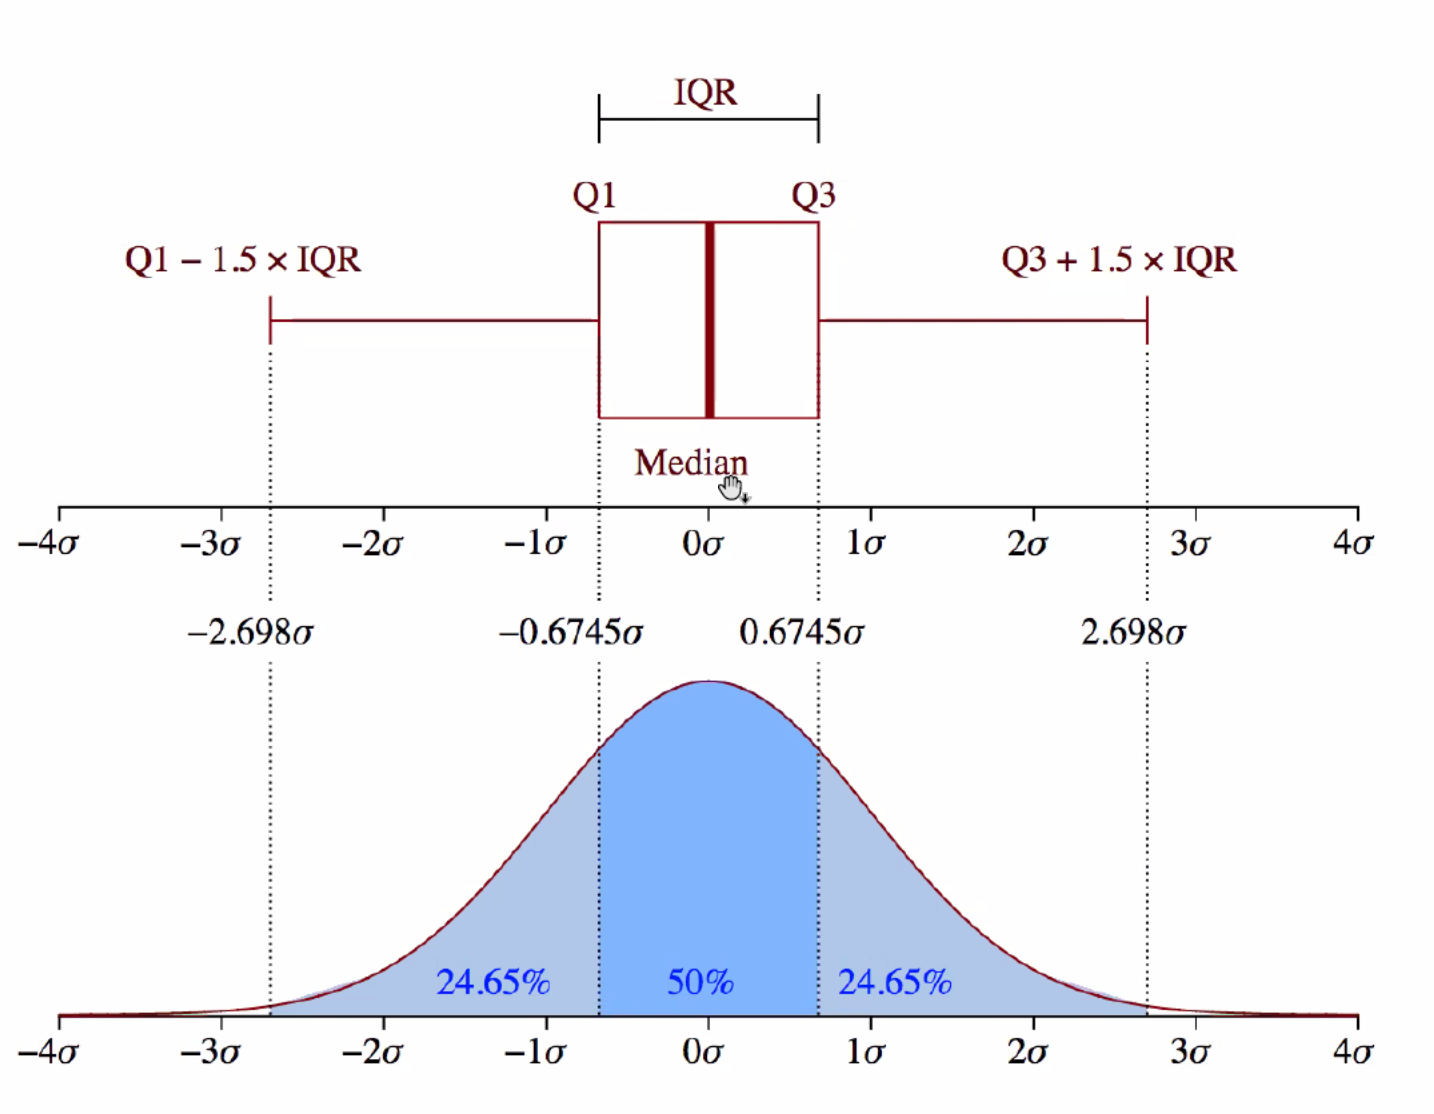
\includegraphics[width=0.7\linewidth]{Images/BoxPlotExample}
            \label{fig:boxplotexample}
        \end{figure}
    \end{remark}
    \paragraph{Выборочные моменты.}
    \begin{definition}
        $\alpha_k=\Expected\xi_1^k$~--- \textbf{$k$-тый теоретический момент}.
    \end{definition}
    \begin{definition}
        $\beta_k=\Expected(\xi_1-\Expected\xi_1)^k$~--- \textbf{$k$-тый центральный теоретический момент}.
    \end{definition}
    \begin{definition}
        Пусть у нас есть $g\colon\mathbb R\to\mathbb R$. Тогда
        \[
        \overline{g(x)}=\frac1n\sum\limits_{k=1}^ng(\xi_k)
        \]
    \end{definition}
    \begin{definition}
        $\widehat{\alpha_k}=\overline{\xi^k}=\frac1n\sum\limits_{j=0}^n\xi_j^k$~--- \textbf{$k$-тый выборочный момент}.
    \end{definition}
    \begin{claim}[несмещённость]
        \[\Expected\widehat{\alpha_k}=\alpha_k\]
    \end{claim}
    \begin{claim}
        \[
        \Variance\widehat{\alpha_k}=\frac1n\Variance\xi_1^k=\frac1n(\Expected\xi_1^{2k}-(\Expected\xi^k)^2)
        \]
    \end{claim}
    \begin{claim}[состоятельность]
        По ЗБЧ
        \[
        \widehat{\alpha_k}\overset p\rightarrow\alpha_k
        \]
    \end{claim}
    \begin{claim}
        Из ЦПТ следует, что
        \[
        \sqrt{n}\frac{\widehat{\alpha_k}-\alpha_k}{\alpha_{2k}-\alpha_k^2}\approx\operatorname{N}(0;1)
        \]
        При этом
        \[
        \sqrt n\frac{\widehat{\alpha_k}-\alpha_k}{\widehat{\alpha_{2k}}-\widehat{\alpha_k}^2}=\sqrt n\frac{\widehat{\alpha_k}-\alpha_k}{\alpha_{2k}-\alpha_k^2}\cdot\frac{\alpha_{2k}-\alpha_k^2}{\widehat{\alpha_{2k}}-\widehat{\alpha_k}^2}
        \]
        Левая часть по распределению стремится у $\operatorname{N}(0;1)$, а правая~--- по вероятности сходится к 1, так как
        \[
        \widehat{\alpha_{2k}}-\widehat{\alpha_k}^2\overset p\longrightarrow\alpha_{2k}-\alpha_k^2
        \]
    \end{claim}
    \begin{definition}
        Также $\overline\xi$ называется \textbf{выборочным средним}.
    \end{definition}
    \begin{remark}
        При выборочном среднем в знаменателе дроби выше написана дисперсия.
    \end{remark}
    \begin{definition}
        $\widehat{\beta_k}=\overline{(\xi-\overline{\xi})^k}=\frac1n\sum\limits_{j=1}^n(\xi_j-\overline\xi)^k$ называется \textbf{$k$-тым центральным выборочным моментом}.
    \end{definition}
    \begin{definition}
        $\widehat{\beta_2}$ называется \textbf{выборочной дисперсией}, а $S_*=\sqrt{\widehat{\beta_2}}$~--- \textbf{выборочным стандартным (среднеквадратичным) отклонением}.
    \end{definition}
    \begin{remark}
        Выборочные моменты есть ни что иное как моменты, посчитанные относительно эмпирического распределения. Отсюда, напрмиер, $S^2_*=\overline{\xi^2}-\overline{\xi}^2$. И куча других формул вида
        \[
        \Expected(\xi-\Expected\xi)^k=\operatorname{poly}(\Expected\xi,\ldots,\Expected\xi^k)
        \]
    \end{remark}
    \begin{claim}
        Из последнего $k$-тый выборочный центральный момент является состоятельной оценкой $k$-того центрального теоретического момента.
    \end{claim}
    \paragraph{Отступление.}
    \begin{claim}
        Пусть $\Xi_n$~--- последовательность случайных векторов. Пусть $\sqrt n(\Xi_n-\mu)\overset d\longrightarrow\operatorname{N}(\mathbb0;\Sigma)$. Тогда $\Xi_n\overset p\rightarrow\mu$.
    \end{claim}
    \begin{proof}
        Ну, $(\Xi_n-\mu)\frac{\sqrt n}{\sqrt n}$ по распределению сходится к нулю, а для вырожденных величин по распределению и по вероятности одно и то же.
    \end{proof}
    \begin{remark}
        Отсюда и далее градиент~--- строка.
    \end{remark}
    \begin{claim}
        Пусть $\phi\in C^1(\mathbb R^m\to\mathbb R)$. Тогда
        \[
        \sqrt n(\phi(\Xi_n)-\phi(\mu))\approx\sqrt n\nabla\phi(\mu)(\Xi_n-\mu)\rightarrow\operatorname{N}(0;\nabla\phi(\mu)\Sigma(\nabla\phi(\mu))^{\mathsf T})
        \]
    \end{claim}
    \begin{proof}
        Тейлор с остатком в Лагранже:
        $\phi(\Xi_n)=\phi(\mu)+\nabla\phi(\tilde{\mu})(\Xi_n-\mu)$. Если $n\to\infty$, то $\nabla\phi(\tilde{\mu})\to\nabla\phi(\mu)$. Отсюда
        \[
        \phi(\Xi_n)-\phi(\mu)\approx\nabla\phi(\mu)(\Xi_n-\mu)
        \]
        и
        \[
        \Variance(\phi(\Xi_n)-\phi(\mu))\approx\Variance(\nabla\phi(\mu)(\Xi_n-\mu))=\Variance(\nabla\phi(\mu)\Xi_n)=\nabla\phi(\mu)\Variance\Xi_n(\nabla\phi(\mu))^{\mathsf T}
        \]
        А отсюда
        \[
        \sqrt n(\phi(\Xi_n)-\phi(\mu))\approx\sqrt n\nabla\phi(\mu)(\Xi_n-\mu)\rightarrow\operatorname{N}(0;\nabla\phi(\mu)\Sigma(\nabla\phi(\mu))^{\mathsf T})
        \]
    \end{proof}
    \begin{definition}
        Всё вышеописанное~--- дельта-метод.
    \end{definition}
    \begin{theorem}
        Многомерная ЦПТ: $\sqrt n(\Xi_n-\alpha)\overline d\rightarrow\operatorname{N}(0;\Sigma)$, где $\alpha=(\alpha_1;\ldots;\alpha_k)$, $\Sigma=\Variance(\xi_1;\ldots;\xi_1^k)$.
    \end{theorem}
    \begin{theorem}
        Пусть $\Xi_n=\left(\overline{\xi},\ldots,\overline{\xi^k}\right)$. Пусть $\phi\in C(\mathbb R^k\to\mathbb R)$. Пусть
        \[
        \sigma=\nabla\phi(\alpha)\Sigma(\nabla\phi(\alpha))^{\mathsf T}
        \]
        Тогда
        \[
        \sqrt n\frac{\phi(\Xi_n)-\phi(\alpha)}{\sigma}\overset d\longrightarrow\operatorname{N}(0;1)
        \]
        Кроме того если $\sigma(\alpha)\in C(\mathbb R^k)$, то
        \[
        \sqrt n\frac{\phi(\Xi_n)-\phi(\alpha)}{\sigma(\Xi_n)}\overset d\longrightarrow\operatorname{N}(0;1)
        \]
    \end{theorem}
    \begin{claim}[Упражнение]
        \[
        \sqrt n\frac{S_*^2-\sigma^2}{\sqrt{\widehat{\beta_4}-S_*^4}}\approx\operatorname{N}(0;1)
        \]
    \end{claim}
    \begin{claim}[Упражнение]
        \[
        \Expected S_*^2=\frac{n-1}n\sigma^2
        \]
    \end{claim}
    \begin{definition}
        \[
        S^2=\frac n{n-1}S_*^2=\frac 1{n-1}\sum\limits_{j=1}^n(\xi_i-\overline \xi)^2
        \]
        называется \textbf{исправленной (несмещённой) дисперсией}.
    \end{definition}
    \begin{definition}
        \textbf{Коэффициент ассиметрии}~--- это $\displaystyle\frac{\Expected(\xi-\Expected\xi)^3}{\sigma^3}$.
    \end{definition}
    \begin{definition}
        \textbf{Выборочный коэффициент ассиметрии}~--- это $\displaystyle\widehat{\gamma}=\frac{\widehat{\beta_3}}{S_*^3}$.
    \end{definition}
    \begin{definition}
        \textbf{Коэффициент эксцесса}~--- это $\displaystyle\frac{\Expected(\xi-\Expected\xi)^4}{\sigma^4}-3$.
    \end{definition}
    \begin{definition}
        \textbf{Выборочный коэффициент эксцесса}~--- это $\displaystyle\frac{\widehat{\beta_4}}{S_*^4}-3$.
    \end{definition}
    \begin{definition}
        Пусть у нас есть выборка $\xi_1,\ldots,\xi_n$ и другая выборка $\eta_1,\ldots,\eta_n$. \textbf{Выборочной ковариацией} называется
        \[
        S_{*\xi\eta}=\frac1n\sum\limits_j\xi_j\eta_j-\overline{\xi}\overline{\eta}=\frac1n\sum\limits_j(\xi_j-\overline\xi)(\eta_j-\overline\eta)
        \]
    \end{definition}
    \begin{definition}
        Выборочным коэффициентом корреляции называется $\displaystyle \rho_n=\frac{S_{*\xi\eta}}{S_{*\xi}S_{*\eta}}$
    \end{definition}
    \section{Порядковые статистики.}
    \begin{definition}
        \textbf{Вариационный ряд}~--- отсортированная по неубыванию выборка. Обозначение: $\xi_{(i)}$.\\
        $\xi_{(k)}$ называется $k$-той порядковой статистикой.
    \end{definition}
    \begin{remark}
        В некоторых книжках вариационный ряд~--- не просто отсортированная, но и сгруппированная по частоте.
    \end{remark}
    \begin{definition}
        \textbf{Квантилью} порядка $\alpha$ называется число $q_\alpha$ такое что
        \[
        P(\xi\geqslant q_\alpha)\geqslant1-\alpha\qquad\qquad P(\xi\leqslant q_\alpha)\geqslant\alpha
        \]
    \end{definition}
    \begin{claim}
        Если функция распределения строго возрастает, $q_\alpha$ определяется единственным образом: $q_\alpha=F^{-1}(\alpha)$.
    \end{claim}
    \begin{claim}
        В противном случае квантилью можно считать либо $\sup\{x\mid F(x)\leqslant\alpha\}$, либо $\inf\{x\mid F(x)\geqslant\alpha\}$.
    \end{claim}
    \begin{definition}
        \textbf{Выборочной квантилью} порядка $0$ называется минимум, \textbf{выборочной квантилью} порядка $q$ называется максимум, выборочной квантилью порядка $\alpha\in(0;1)$ называется вот что.\\
        Заметим, что
        \[
        \exists k\in[0..n-1].\,\frac kn\leqslant\alpha<\frac{k+1}n
        \]
        Тогда $\xi_{(k+1)}$~--- \textbf{выборочная квантиль} порядка $\alpha$.
    \end{definition}
    \begin{definition}
        $q_0$ называется \textbf{нижним квартилем}, $q_{1/4}$~--- \textbf{первый (нижний) квартиль}, $q_{1/2}$~--- \textbf{второй квартиль}, $q_{3/4}$~--- \textbf{третий (верхний) квартиль}, $q_1$~--- \textbf{четвёртый квартиль}.
    \end{definition}
    \begin{definition}
        \textbf{Межквартильный размах} (IQR)~--- $q_{3/4}-q_{1/4}$.
    \end{definition}
    \begin{definition}
        \textbf{Выборочной медианой} называется $\xi_{(m+1)}$, если $n=2m+1$ или $\frac{\xi_{(m)}+\xi_{(m+1)}}2$.
    \end{definition}
    \begin{claim}
        Что значит, что $P(\xi_{(k)}\leqslant t)$? Что
        \[
        P(\mu_n(t)\geqslant k)=\sum\limits_{j=k}^n\binom nk(F(t))^j(1-F(t))^{n-j}=B(F(t);k;n-k+1)
        \]
    \end{claim}
    \begin{definition}
        \textbf{Обобщённой $\beta$-функцией} называется
        \[
        B(z;a;b)=\frac{\Gamma(a+b)}{\Gamma(a)\Gamma(b)}\int\limits_0^zt^{a-1}(1-t)^{b-1}\mathrm dt
        \]
    \end{definition}
    \begin{claim}
        Пусть $p=F'$. Тогда плотность $k$-той порядковой статистики равна
        \[
        \frac{\mathrm d}{\mathrm dt}B(F(t);k;n-k+1)=\frac{\Gamma(n+1)}{\Gamma(k)\Gamma(n-k+1)}(F(t))^{k-1}(1-F(t))^{n-k}p(t)
        \]
    \end{claim}
    \begin{claim}
        Совместная плотность двух порядковых статистик равна
        \[
        g(x_1;x_2)=\frac{n!}{(k-1)!(r-k-1)!(n-r)!}(F(t))^{k-1}(1-F(t))^{r-k-1}p(x_1)p(x_2)
        \]
    \end{claim}
    \begin{claim}
        Совместная плотность всех порядковых статистик равна
        \[
        g(x_1;x_2;\ldots;x_n)=n!p(x_1)p(x_2)\cdots p(x_n)
        \]
    \end{claim}
    \begin{definition}
        Средним членом вариационного ряда называется член с номером $k(n)$: $\frac{k(n)}n\rightarrow\mathrm{const}\in(0;1)$.\\
        Крайний же член вариационного ряда~--- член с номером $r$ (где $r$ ограничено) или с номером $n-1+s$, где $s$ ограничено.
    \end{definition}
    \begin{theorem}[Об асимптотике среднего члена вариационного ряда]
        Пусть $\alpha\in(0;1)$, $q_\alpha$~--- теоретическая квантиль порядка $\alpha$, $p\in C^{(1)}(V_{q_\alpha})$~---теоретическая плотность. И пусть $p(q_\alpha)>0$.\\
        Тогда $\sqrt np(q_\alpha)\frac{\xi_{(\lfloor n\alpha\rfloor)}-q_\alpha}{\sqrt{\alpha(1-\alpha)}}\overset d\longrightarrow\operatorname{N}(0;1)$
    \end{theorem}
    \begin{proof}
        Идея доказательства: пусть $k=\lfloor n\alpha\rfloor$. Пусть $g(x)=\sqrt np(q_\alpha)\frac{x-q_\alpha}{\sqrt{\alpha(1-\alpha)}}$. Напишем плотность этого:
        \[
        p_{g(\xi_{(k)})}(t)=p_{\xi_{(k)}}(g^{-1}(t))\cdot g^{-1}(t)'_t
        \]
        Дальше надо расписать всё по Стирлингу, и в пределе будет что надо.
    \end{proof}
    \begin{example}
        Пусть у нас $\operatorname{Cauchy}(\mu;1)$, $\alpha=\frac12$. Тогда
        \[
        p(\mu)\sqrt n2(\xi_{(\lfloor\frac n2\rfloor)}-\mu)=\frac1\pi\frac1{1+(\mu-\mu)^2}2\sqrt n(\xi_{(\lfloor\frac n2\rfloor)}-\mu)
        \]
    \end{example}
    \begin{theorem}[Об асимптотике крайних членов вариационного ряда]
        Пусть $p$~--- плотность. Тогда
        \[
        nF(\xi_{(r)})\overset d\longrightarrow\operatorname{\Gamma}(r;1)
        \]
        \[
        nF(\xi_{(n+1-s)})\overset d\longrightarrow\operatorname{\Gamma}(s;1)
        \]
        Кроме того $\operatorname{\Gamma}(r;1)$ и $\operatorname{\Gamma}(s;1)$ независимы
    \end{theorem}
    \section{Постановка задачи точечного оценивания параметров.}
    \begin{remark}
        Пусть у нас $\xi_1;\ldots;\xi_n$ имеют распределение $\theta$, где $\theta\in\Theta\subset\mathbb R^{d}$. И $\theta$~--- фиксированный неизвестный вектор.\\
        Наша цель~--- оценить $\theta$ в виде $\widehat{\theta}=\widehat{\theta}(\xi_1;\ldots;\xi_n)$ (в виде функции от выборки).
    \end{remark}
    \begin{definition}
        \textbf{Статистика}~--- измеримая функция от выборки.
    \end{definition}
    \begin{remark}
        Ещё есть Байесовская постановка задачи: там $\theta$~--- случайная величина из известного распределения $\Theta$.
    \end{remark}
    \begin{definition}
        Говорят, что $\widehat{\theta}$~--- \textbf{состоятельная оценка} $\theta$, если $\widehat{\theta}\overset d\longrightarrow\theta$.
    \end{definition}
    \begin{definition}
        \textbf{Смещением} называется $\operatorname{bias}(\widehat\theta)=\Expected\widehat{\theta}-\theta$.
    \end{definition}
    \begin{definition}
        Если смещение равно нулю, оценка называется \textbf{несмещённой}.
    \end{definition}
    \begin{definition}
        Если смещение стремится к нулю, оценка называется \textbf{асимптотически несмещённой}.
    \end{definition}
    \begin{definition}
        Оценка $\widehat\theta$ \textbf{асимптотически нормальна}, если
        \[
        \sqrt n(\widehat{\theta}-\theta)\rightarrow\operatorname{N}(0;\Sigma)
        \]
    \end{definition}
    \begin{example}
        Пусть у нас есть $\operatorname{Bern}(p)$, и мы не знаем $p$. Каким мы хотим его взять? Ну, например $\overline\xi$. Тогда по ЗБЧ она состоятельна, очевидно несмещена и по ЦПТ асимптотически нормальна.
    \end{example}
    \begin{example}
        Пусть у нас $\operatorname{N}(\mu;\sigma^2)$. И пусть $\mu$ мы знаем, а $\sigma^2$~--- нет. Кто мы берём? Например, $S_*^2$. Но увы, эта оценка смещена. Только асимптотическая несмещённость есть.
    \end{example}
    \begin{definition}
        Будем говорить, что $\widehat{\theta}_1$ оптимальнее (эффективнее) $\widehat{\theta}_2$, если
        \[
        \operatorname{MSE}(\widehat{\theta}_1)<\operatorname{MSE}(\widehat{\theta}_2)
        \]
        Где
        \[
        \operatorname{MSE}(\widehat{\theta})=\Expected\|\widehat\theta-\theta\|^2=\Expected(\widehat\theta-\theta)^{\mathsf T}(\widehat\theta-\theta)
        \]
    \end{definition}
    \begin{remark}
        В некоторых книжках эти понятия различны, но у нас они будут одним.
    \end{remark}
    \begin{claim}
        Если $\widehat{\theta}$ несмещена
        \[
        \operatorname{MSE}(\widehat{\theta})=\tr(\Variance\widehat{\theta})+\|\operatorname{bias}\widehat{\theta}\|^2
        \]
    \end{claim}
    \begin{proof}
        Тут надо воспользоваться тем, что $\theta=\Expected\widehat{\theta}$.
    \end{proof}
\end{document}
